% !TEX root = ./main.tex
% ^ Tells LaTeX Workshop (Cursor/VSCode) to treat this file as the build root.
% Needed because \documentclass lives in arena_beamer.sty (\input'ed below)
% rather than in this file, and the extension's root-file detector greps for
% \documentclass without following \input -- so without this line it reports
% "No root file found" and silently aborts Ctrl+Alt+B. CLI builds are
% unaffected; latexmk/pdflatex follow \input fine.
% Local-dev build-mode toggle. 1 = handout (all \pause overlays collapsed,
% small PDF), 0 = presentation (each \pause becomes an extra page, for
% live talks). CI overrides this via latexmk -usepretex regardless of what
% it's set to here, so this line only affects local pdflatex/latexmk runs.
\providecommand{\HANDOUT}{1}
\input{../../arena_beamer.sty}

% Deck-local macros (RL chapter math notation).
\newcommand{\A}{\mathcal{A}}
\newcommand{\eps}{\epsilon}
\newcommand{\pth}{{\boldsymbol{\phi}}}
\newcommand{\old}{\text{old}}
\newcommand{\refm}{\text{ref}}
\newcommand{\piold}{\pi_{\bth_\old}}
\newcommand{\piref}{\pi_\refm}
\newcommand{\KL}{D_{\mathrm{KL}}}
% log-ratio to the reference model; deliberately not rho, which is the
% importance ratio to the old policy (as in the PPO deck)
\newcommand{\lr}{u}

\begin{document}

\title[{[2.4] RLHF \& RLVR}]
{{[2.4] RLHF \& RLVR}}

\author[David Quarel]
{David Quarel}

\institute[ARENA]
{
  ARENA
}

\date[\today]
{\today}

\frame{\titlepage}

% ============================================================
\section{Where we left off}

\begin{frame}
    \frametitle{Recap: PPO}
    \begin{block}{PPO clipped joy}
        $$
        J^{CLIP}(\bth) = \hat{\Ex}_t\Big[\min\big(\rho_t(\bth)\,\red{A_t},\;
        \text{clip}(\rho_t(\bth), 1-\eps, 1+\eps)\,\red{A_t}\big)\Big],
        \qquad
        \rho_t(\bth) = \frac{\pi_\bth(a_t|s_t)}{\piold(a_t|s_t)}
        $$
    \end{block}
    \begin{itemize}
        \item \red{$A_t$} came from a \textbf{critic} $V_\pth$ and GAE.
        \item Clipping lets us reuse each batch for several gradient steps.
        \item An entropy bonus kept the policy exploring.
    \end{itemize}
    \pause
    \vspace{0.3cm}
    Today: point this at a \textbf{language model}.
    \begin{enumerate}
        \item \textbf{RLHF}: reward from a learned model of what humans like. \hfill $\to$ \textbf{GRPO + KL}
        \item \textbf{LoRA}: fine-tune a model too big to fit. \hfill $\to$ \textbf{train a low-rank update}
        \item \textbf{RLVR}: reward from a checker. \hfill $\to$ \textbf{Dr.\ GRPO + curriculum}
    \end{enumerate}
\end{frame}

% ============================================================
\section{The language model as an environment}

\begin{frame}
    \frametitle{States, actions, rewards}
    \begin{itemize}
        \item \textbf{Policy} $\pi_\bth$: the language model.
        \item \textbf{Action} $a_t$: the next token. $\A$ is the vocabulary.
        \item \textbf{State} $s_t$: the \textit{whole} sequence so far, $s_t = s_0\, a_0 \ldots a_{t-1}$.
        \item \textbf{Dynamics}: concatenate, $s_{t+1} = s_t\, a_t$. Deterministic.
    \end{itemize}
    \begin{center}
    \begin{tikzpicture}[tok/.style={draw, thick, rounded corners, minimum height=7mm, font=\small},
        node distance=1.5mm]
        \node[tok, fill=gray!15] (p) {\texttt{This is}};
        \node[tok, fill=red!10, right=of p] (a0) {\texttt{\ a}};
        \node[tok, fill=red!10, right=of a0] (a1) {\texttt{\ conversation}};
        \node[tok, fill=red!10, right=of a1] (a2) {\texttt{\ between}};
        \node[right=of a2] (dots) {$\cdots$};
        \node[tok, fill=red!10, right=of dots] (aT) {\texttt{.}};
        \node[below=1mm of p, font=\scriptsize] {$s_0$ (prompt)};
        \node[below=1mm of a0, font=\scriptsize] {$a_0$};
        \node[below=1mm of a1, font=\scriptsize] {$a_1$};
        \node[below=1mm of a2, font=\scriptsize] {$a_2$};
        \node[below=1mm of aT, font=\scriptsize] {$a_{T-1}$};
        \node[blue, right=4mm of aT, align=left, font=\small] (r) {$r_T = R(s_T)$};
        \draw[->, thick, blue] (aT) -- (r);
    \end{tikzpicture}
    \end{center}
    \pause
    \begin{itemize}
        \item \textbf{Reward}: $0$ on every step, except the last: $r_T = R(s_0 a_0 \ldots a_{T-1})$.
        \item Fixed length $T$, one reward at the end: discounting only multiplies everything by
        $\gamma^{T-1}$, so we \textbf{don't discount}. Return $=$ reward.
        \item We never visit the same state twice. All the difficulty is in $R$.
    \end{itemize}
\end{frame}

% ============================================================
\section{GRPO}

\begin{frame}
    \frametitle{Do we need a critic?}
    PPO's advantage needs $V(s_t)$. For a language model, that means:
    \begin{itemize}
        \item Graft a \textbf{value head} onto the residual stream, mapping it to a scalar.
        \item It starts random, and must learn the value of a half-written sentence.
        \item Extra parameters, extra memory, extra things to tune.
    \end{itemize}
    \pause
    \vspace{0.2cm}
    \textbf{GRPO} (DeepSeekMath, 2024): skip the critic.
    \begin{itemize}
        \item Sample a \textbf{group} of $G$ completions $o_1, \ldots, o_G$ of the same prompt $q$.
        \item Use the group's average reward as the baseline.
    \end{itemize}
    \begin{block}{Group-relative advantage}
        $$
        \hat{A}_i = \frac{r_i - \operatorname{mean}(r_1, \ldots, r_G)}{\operatorname{std}(r_1, \ldots, r_G)}
        $$
    \end{block}
    \pause
    \begin{itemize}
        \item Baseline depends only on the prompt, not the action: free (PPO deck).
        \item Every token of $o_i$ gets the \textit{same} advantage $\hat{A}_i$.
    \end{itemize}
\end{frame}

\begin{frame}
    \frametitle{A group, scored}
    \begin{center}
    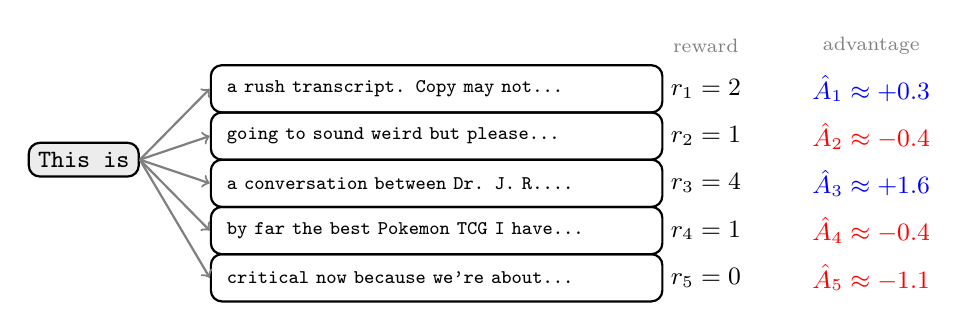
\begin{tikzpicture}[
        comp/.style={draw, thick, rounded corners, minimum height=6mm, text width=55mm, font=\scriptsize\ttfamily, align=left},
        node distance=1.2mm]
        \node[draw, thick, rounded corners, fill=gray!15, font=\small\ttfamily] (q) at (0,0) {This is};
        \foreach \i/\txt/\r/\a/\col in {
            1/{\ a rush transcript. Copy may not\ldots}/2/{+0.3}/blue,
            2/{\ going to sound weird but please\ldots}/1/{-0.4}/red,
            3/{\ a conversation between Dr. J. R.\ldots}/4/{+1.6}/blue,
            4/{\ by far the best Pokemon TCG I have\ldots}/1/{-0.4}/red,
            5/{\ critical now because we're about\ldots}/0/{-1.1}/red} {
            \node[comp, anchor=west] (o\i) at (1.6, 1.5 - 0.6*\i) {\txt};
            \node[font=\small] (r\i) at (7.9, 1.5 - 0.6*\i) {$r_\i = \r$};
            \node[font=\small, \col] at (10.0, 1.5 - 0.6*\i) {$\hat{A}_\i \approx \a$};
            \draw[->, thick, gray] (q.east) -- (o\i.west);
        }
        \node[font=\scriptsize, gray] at (7.9, 1.45) {reward};
        \node[font=\scriptsize, gray] at (10.0, 1.45) {advantage};
    \end{tikzpicture}
    \end{center}
    \small
    Reward = number of periods. Mean $1.6$, std $1.5$. (Illustrative group of 5; the real one is 128.)
    \pause
    \begin{itemize}
        \item Better than the group: \blue{push every token up}. Worse: \red{push every token down}.
        \item \textbf{Every reward the same?} Then every $\hat{A}_i = 0$, and the group teaches nothing.
        We need diversity within a group.
        \pause
        \item \textbf{Many prompts?} Normalise \textit{within} each prompt's group.
        Otherwise we learn ``easy prompts are good'', which the policy can't act on.
    \end{itemize}
\end{frame}

\begin{frame}
    \frametitle{The GRPO objective}
    \begin{block}{GRPO joy (maximise)}
        $$
        J^{GRPO}(\bth) = \Ex\Bigg[\frac{1}{G}\sum_{i=1}^G \frac{1}{|o_i|}\sum_{t=1}^{|o_i|}
        \Big(
        \underbrace{J^{CLIP}_{i,t}(\bth)}_{\text{PPO's clipped joy}}
        - \beta\, \underbrace{\KL\big[\pi_\bth \,\|\, \piref\big]}_{\text{new}}
        \Big)\Bigg]
        $$
    \end{block}
    with
    $$
    J^{CLIP}_{i,t} = \min\big[\rho_{i,t}\hat{A}_i,\ \text{clip}(\rho_{i,t}, 1-\eps, 1+\eps)\,\hat{A}_i\big],
    \qquad
    \rho_{i,t} = \frac{\pi_\bth(o_{i,t} \mid q, o_{i,<t})}{\piold(o_{i,t} \mid q, o_{i,<t})}.
    $$
    \pause
    \vspace{0.3cm}
    \begin{center}
    \renewcommand{\arraystretch}{1.3}
    \begin{tabular}{l|l|l}
                       & \textbf{PPO} & \textbf{GRPO} \\ \hline
        advantage      & critic + GAE, per step & group baseline, per sequence \\
        clipping       & $\text{clip}(\rho_t)$ & same \\
        regulariser    & entropy bonus & KL to the original model $\piref$ \\
        extra network  & critic $V_\pth$ & frozen copy $\piref$
    \end{tabular}
    \end{center}
\end{frame}

% ============================================================
\section{The KL penalty}

\begin{frame}
    \frametitle{Why a KL penalty?}
    \begin{itemize}
        \item In RLHF, $R$ is a \textbf{model} of human preferences: a proxy.
        Optimise a proxy hard enough and it breaks.
        \item The policy can find text that $R$ loves but no human would write.
        \item So: maximise reward, but stay close to the pretrained model $\piref$.
    \end{itemize}
    \pause
    \vspace{0.2cm}
    \textbf{Which direction?} We use $\KL(\pi_\bth \,\|\, \piref)$, the \textbf{reverse} KL.
    \begin{columns}
    \begin{column}{0.48\linewidth}
    \begin{itemize}
        \item Blows up where $\pi_\bth$ puts mass and $\piref$ doesn't: no new garbage.
        \item Fine for $\pi_\bth$ to \textit{drop} things $\piref$ does: we want that!
        \item $\pi_\bth$ \textbf{concentrates} on part of what $\piref$ already does.
    \end{itemize}
    \end{column}
    \begin{column}{0.5\linewidth}
    \centering
    \includegraphics[width=\linewidth]{kl_diff}
    {\tiny Red: $P$. Blue: the Gaussian $Q$ fit to it. Right panel = mode-seeking.}
    \end{column}
    \end{columns}
\end{frame}

\begin{frame}
    \frametitle{The exact KL is expensive}
    Per position, sum over the vocabulary:
    $$
    \KL\big(\pi_\bth(\cdot|s_t) \,\|\, \piref(\cdot|s_t)\big)
    = \sum_{a \in \A} \pi_\bth(a|s_t) \log \frac{\pi_\bth(a|s_t)}{\piref(a|s_t)}
    $$
    \pause
    \begin{itemize}
        \item Needs $\piref$'s logprobs for \textit{every} token in the vocab, at every position.
        \item GPT-2: $128 \text{ samples} \times 30 \text{ tokens} \times 50\text{k vocab} \times 4\text{ bytes} \approx 740$ MiB, just to store it.
        \item Qwen's vocab is $152$k. Gemma 3's is $262$k.
        \pause
        \item Most of the mass is on a handful of tokens anyway.
    \end{itemize}
    \pause
    \vspace{0.2cm}
    KL is an expectation under $\pi_\bth$, and we \textit{already have samples} from (roughly) $\pi_\bth$:
    the tokens we generated. Estimate it from the \textbf{sampled token only}.
    Let
    $$
    \lr_t = \log \pi_\bth(a_t|s_t) - \log \piref(a_t|s_t).
    $$
\end{frame}

\begin{frame}
    \frametitle{Three estimators}
    \begin{center}
    \renewcommand{\arraystretch}{1.5}
    \begin{tabular}{l|c|c|c}
         & \textbf{k1} & \textbf{k2} & \textbf{k3} \\ \hline
        formula & $\lr_t$ & $\tfrac12 \lr_t^2$ & $e^{-\lr_t} - 1 + \lr_t$ \\
        unbiased? & yes & no (small bias) & yes \\
        always $\ge 0$? & no & yes & yes \\
        variance & huge & low & low \\
        \onslide<2->{\red{expected gradient}} & \onslide<2->{\red{$0$}} & \onslide<2->{\red{$\nabla \KL(\pi_\bth\|\piref)$}} & \onslide<2->{\red{$\nabla \KL(\piref\|\pi_\bth)$}}
    \end{tabular}
    \end{center}
    \vspace{0.2cm}
    \begin{itemize}
        \item k3 is the best \textit{measurement} of the KL (Schulman).
        It's what the GRPO paper and TRL use.
        \pause
        \item But we don't use the penalty's value, we \textbf{differentiate} it.
        For a penalty $k(\lr_t)$, the expected gradient is
        $\Ex_{a\sim\pi_\bth}\big[k'(\lr)\,\nabla_\bth \log \pi_\bth(a|s)\big]$.
        \item k1 has zero expected gradient, and k3's is the gradient of the \textit{forward} KL:
        the direction we just argued against.
        \pause
        \item \textbf{k2} is biased as a measurement, but its gradient is exactly the one we want.
        We train with k2, and log k1 (averaged over the batch) to monitor drift.
    \end{itemize}
\end{frame}

\begin{frame}
    \frametitle{Where did the entropy bonus go?}
    $$
    \KL(\pi_\bth \,\|\, \piref)
    = \underbrace{\sum_a \pi_\bth \log \pi_\bth}_{-H(\pi_\bth)}
    \;\underbrace{- \sum_a \pi_\bth \log \piref}_{\text{cross-entropy}}
    $$
    \pause
    \begin{itemize}
        \item Penalising the KL already \textbf{rewards entropy}.
        \item And it pulls $\pi_\bth$ towards a pretrained model, which spreads its mass over
        many plausible continuations.
        \item Usually enough to stop collapse, without a separate bonus.
    \end{itemize}
\end{frame}

% ============================================================
\section{Training}

\begin{frame}
    \frametitle{The GRPO training loop}
    \textbf{Repeat for each phase:}
    \begin{enumerate}
        \item \textbf{Rollout:} sample $G$ completions of the prompt from $\pi_\bth$ (no truncation:
        \texttt{top\_k=0}, \texttt{top\_p=1}). Compute rewards and $\hat{A}_i$.
        \item \textbf{Learn:} for each epoch, for each shuffled minibatch:
        rerun $\pi_\bth$ on the samples, ascend $J^{CLIP} - \beta\,\text{k2}$.
    \end{enumerate}
    \pause
    \vspace{0.2cm}
    \begin{center}
    \small
    \renewcommand{\arraystretch}{1.3}
    \begin{tabular}{l|l}
        \textbf{Stored during rollout} & \textbf{Recomputed per minibatch} \\ \hline
        token ids (the actions are inside them) & $\log \pi_\bth(o_{i,t}|\ldots)$ \\
        $\log \piold(o_{i,t}|\ldots)$, for $\rho_{i,t}$ & \\
        $\log \piref(o_{i,t}|\ldots)$, for the KL & \\
        $\hat{A}_i$, one per sequence & \\ \hline
        \textit{frozen: just numbers} & \textit{live: carries gradients}
    \end{tabular}
    \end{center}
    \pause
    \begin{itemize}
        \item Only logprobs of \textit{sampled} tokens: $(G, T)$, not $(G, T, |\A|)$.
        \item Keep the model in \texttt{.eval()}: dropout would make $\rho$ noisy and not start at $1$.
    \end{itemize}
\end{frame}

\begin{frame}
    \frametitle{Reward: count the periods}
    \textbf{$\beta = 0$} (no KL penalty). Within 4 phases:
    \begin{center}
    \texttt{\small This is.........................................}
    \end{center}
    Every sample identical $\Rightarrow$ every $\hat{A}_i = 0$ $\Rightarrow$ training stops. Reward $90$.
    \pause
    \vspace{0.3cm}

    \textbf{$\beta > 0$}: the model has to launder periods into plausible text.
    \begin{itemize}
        \item \texttt{\small This is a rush transcript. Copy may not be in its final form.}
        \item \texttt{\small This is a conversation between Dr. Fedora . . . . . .}
        \item \texttt{U.S.}, \texttt{Python 2.7.12}, \texttt{C. S. Lewis}, \texttt{9.5cm x 7.5 cm}, \ldots
    \end{itemize}
    \pause
    \vspace{0.2cm}
    \textbf{Why doesn't the KL stop ``\texttt{. . . . .}''?}
    \begin{itemize}
        \item The KL compares the two models \textit{in the same context}.
        \item After \texttt{. . . .}, the base model also predicts another \texttt{.}
        \item Only the first few tokens of the pattern pay the penalty.
    \end{itemize}
\end{frame}

% ============================================================
\section{LoRA}

\begin{frame}
    \frametitle{Full fine-tuning doesn't fit}
    AdamW in float32, per parameter:
    \begin{center}
    \begin{tabular}{lr}
        weight & 4 bytes \\
        gradient & 4 bytes \\
        Adam's two moments & 8 bytes \\ \hline
        \textbf{total} & \textbf{16 bytes}
    \end{tabular}
    \end{center}
    \pause
    For Qwen3-1.7B: $1.7\text{B} \times 16 \approx \red{27\text{ GB}}$, plus $\red{7\text{ GB}}$ for the frozen $\piref$.
    Before a single activation. A 24 GB GPU can't do it.
    \pause
    \vspace{0.3cm}

    \textbf{But RL barely changes the model.}
    \begin{itemize}
        \item A 0/1 reward gives at most $1$ bit per rollout.
        \item $100$ phases $\times\ 128$ rollouts $= 12{,}800$ bits $\approx 1.5$ KiB, total.
        \item We're nudging a pretrained model towards behaviour it mostly already has.
        Why pay to update every weight?
    \end{itemize}
\end{frame}

\begin{frame}
    \frametitle{Low-Rank Adaptation}
    \begin{columns}
    \begin{column}{0.58\linewidth}
    Freeze $W_0 \in \mathbb{R}^{d_\text{in} \times d_\text{out}}$. Learn a \textbf{low-rank update}:
    \begin{block}{LoRA}
        $$
        h = x W_0 + \frac{\alpha}{r}\, x A B
        $$
        $A \in \mathbb{R}^{d_\text{in} \times r}$, $B \in \mathbb{R}^{r \times d_\text{out}}$, $r \ll d$
    \end{block}
    \pause
    \begin{itemize}
        \item $A$ random, $B = 0$: starts as \textit{exactly} the base model.
        \item Params: $r(d_\text{in} + d_\text{out})$ instead of $d_\text{in} d_\text{out}$.
        Qwen3-1.7B, $r = 8$: well under $1\%$.
        \item Compute $(xA)B$, never $AB$: stay in the rank-$r$ bottleneck.
        \item Adapters in fp32, base in bf16: tiny Adam steps don't round away.
    \end{itemize}
    \end{column}
    \begin{column}{0.4\linewidth}
    \centering
    \includegraphics[width=0.85\linewidth]{LoraDiagram}
    \end{column}
    \end{columns}
\end{frame}

\begin{frame}
    \frametitle{What LoRA buys us}
    \begin{itemize}
        \item \textbf{Optimiser state only for $A, B$}. $W_0$ gets no gradient and no Adam moments.
        \pause
        \item \textbf{Gradients still flow \textit{through} $W_0$}:
        $\frac{\partial L}{\partial x} = \frac{\partial L}{\partial h} W_0^\top$ uses $W_0$'s value,
        never $\frac{\partial L}{\partial W_0}$. Still a full backward pass.
        \pause
        \item \textbf{The reference model is free}: switch the adapters off and you have $\piref$ back.
        No second copy.
    \end{itemize}
    \pause
    \begin{block}{Merging}
        After training, bake it in: $W \leftarrow W_0 + \frac{\alpha}{r} AB$. Same speed as the base model.
    \end{block}
    \begin{itemize}
        \item In bf16, $W_0 + \frac{\alpha}{r}AB$ rounds to $\sim$1 part in 256 of $W_0$.
        Our update is $<1\%$ of $W_0$: merging loses about a quarter of it.
        \item Servers with many adapters (vLLM, S-LoRA) don't merge at all.
    \end{itemize}
    \pause
    \vspace{0.1cm}
    \textbf{Which layers?} Paper: $W_Q, W_V$. Current practice: \textit{every} linear layer,
    attention \textit{and} MLP. For RL, even $r = 1$ can match full fine-tuning.
\end{frame}

% ============================================================
\section{RLVR}

\begin{frame}
    \frametitle{From preferences to verifiers}
    \textbf{RLVR}: Reinforcement Learning from \textbf{Verifiable} Rewards.
    \begin{itemize}
        \item The reward is a \textbf{checker} with access to ground truth:
        a known answer, a calculator, unit tests, a proof checker.
        \item Have the model think out loud (chain of thought), then grade only the final answer.
    \end{itemize}
    \pause
    \vspace{0.2cm}
    \begin{center}
    \renewcommand{\arraystretch}{1.3}
    \begin{tabular}{l|l|l}
         & \textbf{RLHF} & \textbf{RLVR} \\ \hline
        reward & learned proxy for humans & checks the answer \\
        reward hacking & a real worry & mostly not possible\textsuperscript{*} \\
        KL to $\piref$ & essential & \textbf{dropped} \\
        goal & change \textit{behaviour} & teach a \textit{capability}
    \end{tabular}
    \end{center}
    \pause
    \begin{itemize}
        \item If the model learns something it couldn't do before,
        its successful rollouts \textit{must} be out of distribution for $\piref$.
        So we don't want to anchor to $\piref$.
        \item \textsuperscript{*}As long as the checker is right. (Is it ever?)
    \end{itemize}
\end{frame}

\begin{frame}
    \frametitle{The task: multiplication}
    \begin{block}{Prompt}
        \texttt{\small Compute 948 * 39. Reason step by step, then give the final answer as $\backslash$boxed\{N\}.}
    \end{block}
    \begin{itemize}
        \item Trivial to verify, huge input space (no memorising), \textbf{tunable difficulty}.
        \item Qwen3-0.6B-Base knows \textit{how} to multiply, but slips on big numbers.
    \end{itemize}
    \begin{center}
    \small
    \renewcommand{\arraystretch}{1.2}
    \begin{tabular}{l|cccccc}
        rung & 3$\times$2 & 4$\times$2 & 3$\times$3 & 4$\times$3 & 4$\times$4$^\dagger$ & 4$\times$4 \\ \hline
        base pass@1 & 0.56 & 0.44 & 0.30 & 0.16 & 0.08 & 0.05
    \end{tabular}

    {\tiny $^\dagger$second operand $< 3000$. Two more rungs (4$\times$5, 5$\times$5) above these.}
    \end{center}
    \pause
    \begin{columns}
    \begin{column}{0.45\linewidth}
    \begin{block}{Reward}
        \vspace{-0.3cm}
        $$
        r_T = \begin{cases}
            1 & \text{boxed answer correct} \\
            0.1 & \text{boxed, but wrong} \\
            0 & \text{no boxed integer}
        \end{cases}
        $$
    \end{block}
    \end{column}
    \begin{column}{0.5\linewidth}
    \begin{itemize}
        \item The $0.1$ teaches the format fast.
        \item Anything fancier (partial credit, ``close enough''): expect it to be gamed.
    \end{itemize}
    \end{column}
    \end{columns}
\end{frame}

\begin{frame}
    \frametitle{Dr.\ GRPO: drop the std}
    GRPO divides each group's advantages by its std. For 0/1 rewards in a group of 19:
    \vspace{0.2cm}
    \begin{center}
    \renewcommand{\arraystretch}{1.3}
    \begin{tabular}{l|c|c}
        group & std & effect of $/\text{std}$ \\ \hline
        1 right, 18 wrong (too hard) & $0.23$ & \red{amplified $\times 4.4$} \\
        18 right, 1 wrong (too easy) & $0.23$ & \red{amplified $\times 4.4$} \\
        10 right, 9 wrong (just right) & $0.51$ & amplified $\times 2.0$
    \end{tabular}
    \end{center}
    \pause
    \begin{itemize}
        \item Questions that are nearly always solved, or nearly always failed,
        get the \textit{biggest} weight. The questions in the sweet spot get the least.
        \item \textbf{Dr.\ GRPO} (``GRPO Done Right''): just $\hat{A}_i = r_i - \operatorname{mean}(r_1, \ldots, r_G)$.
    \end{itemize}
\end{frame}

\begin{frame}
    \frametitle{Dr.\ GRPO: drop the length normalisation}
    Completions now stop at the end-of-text token, so lengths $|o_i|$ differ.
    $$
    \frac{1}{G}\sum_{i=1}^G \red{\frac{1}{|o_i|}} \sum_{t=1}^{|o_i|} (\ldots)
    \qquad \longrightarrow \qquad
    \frac{1}{G}\sum_{i=1}^G \blue{\frac{1}{L_\text{max}}} \sum_{t=1}^{|o_i|} (\ldots)
    $$
    \pause
    \begin{itemize}
        \item Every token of $o_i$ has the same $\hat{A}_i$, so with $\red{1/|o_i|}$
        each token is pushed by $\hat{A}_i / |o_i|$.
        \item $\hat{A}_i > 0$: short correct answers get a bigger push per token. \hfill $\to$ prefers \textbf{short right}
        \item $\hat{A}_i < 0$: long wrong answers get a smaller penalty per token. \hfill $\to$ prefers \textbf{long wrong}
        \pause
        \item Dr.\ GRPO divides by a \blue{constant}: $L_\text{max}$ = the generation budget (\texttt{max\_new\_tokens}).
        \item New detail: a \textbf{mask} over the tokens up to and including the first EOS.
        (Qwen's pad token \textit{is} EOS, so don't mask by \texttt{!= pad}: the model would never learn to stop.)
    \end{itemize}
\end{frame}

\begin{frame}
    \frametitle{A dynamic curriculum}
    A question with solve rate $p$: how much does one answer tell us?
    \begin{columns}
    \begin{column}{0.5\linewidth}
    $$
    \mathcal{H}(p) = -p\log_2 p - (1-p)\log_2(1-p)
    $$
    \begin{itemize}
        \item Max $1$ bit at $p = 0.5$.
        \item $p = 0$ or $1$: every reward the same, $\hat{A} = 0$, wasted.
    \end{itemize}
    \end{column}
    \begin{column}{0.48\linewidth}
    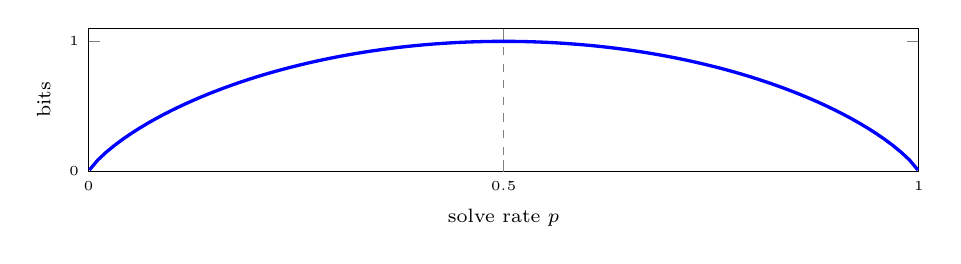
\begin{tikzpicture}
    \begin{axis}[
        width=\linewidth, height=3.4cm,
        xmin=0, xmax=1, ymin=0, ymax=1.1,
        xlabel={solve rate $p$}, ylabel={bits},
        xtick={0,0.5,1}, ytick={0,1},
        tick label style={font=\tiny}, label style={font=\scriptsize}]
        \addplot[very thick, blue, domain=0.001:0.999, samples=100]
            {-x*ln(x)/ln(2) - (1-x)*ln(1-x)/ln(2)};
        \draw[dashed, gray] (axis cs:0.5,0) -- (axis cs:0.5,1);
    \end{axis}
    \end{tikzpicture}
    \end{column}
    \end{columns}
    \pause
    But the model improves, so a fixed difficulty is too hard early and too easy late.
    \begin{block}{Curriculum: track the frontier}
        $$
        D \leftarrow \text{clamp}\big(D + \alpha\,(\hat{s} - 0.5),\ D_\text{min},\ D_\text{max}\big)
        $$
    \end{block}
    \begin{itemize}
        \item $\hat{s}$: this batch's solve rate. Too easy $\to$ harder; too hard $\to$ easier.
        \item $D$ is real-valued; rungs are integers. \textbf{Stochastic rounding}:
        $D = 2.3$ poses rung 2 with prob.\ $0.7$, rung 3 with prob.\ $0.3$.
    \end{itemize}
\end{frame}

\begin{frame}
    \frametitle{One step per rollout}
    RLVR trainer: sample $16$ problems $\times\ 8$ completions, take \textbf{one} optimiser step, discard.
    \pause
    \begin{itemize}
        \item The policy that sampled the batch \textit{is} the one we're updating: $\piold = \pi_\bth$.
        \item Pass $\texttt{old\_logprobs} = \texttt{logprobs.detach()}$:
        $\rho = 1$ in value, but $\nabla_\bth \rho = \nabla_\bth \log \pi_\bth$.
        (Plain \texttt{logprobs} would give $\rho \equiv 1$ and no gradient at all.)
        \item $\rho = 1$ is inside $[1-\eps, 1+\eps]$, so the clip never fires:
    \end{itemize}
    $$
    \nabla_\bth J = \frac{1}{G L_\text{max}} \sum_{i=1}^G \big(r_i - \bar{r}\big)
    \sum_t \nabla_\bth \log \pi_\bth(o_{i,t} \mid q, o_{i,<t})
    $$
    \textbf{REINFORCE with a group-mean baseline.} Back to VPG!
    \pause
    \vspace{0.2cm}

    Why keep the clip then? In general you \textit{do} go off-policy:
    \begin{itemize}
        \item several minibatch steps per rollout (as in our RLHF trainer: $4 \times 2 = 8$),
        \item reusing expensive long rollouts,
        \item the sampler (vLLM) and trainer give slightly different probabilities for the same weights.
    \end{itemize}
\end{frame}

\begin{frame}
    \frametitle{Making it fit}
    \begin{itemize}
        \item RLHF: $128 \times 30 \times 50\text{k} \approx 0.2$B logits, $0.7$ GiB. Fine.
        \item RLVR: $128 \times {\sim}450 \times 152\text{k} \approx 9$B logits, ${\sim}33$ GiB in fp32. \red{Not fine.}
    \end{itemize}
    \pause
    \vspace{0.2cm}
    None of this changes the maths:
    \begin{itemize}
        \item \textbf{Gradient accumulation}: micro-batches of $4$ completions $\to$ ${\sim}1.2$ GiB of logits.
        One optimiser step at the end.
        \item \textbf{Skip zero-advantage rows}: groups where everyone got the same reward contribute exactly $0$.
        \item \textbf{Length-sorted micro-batches}: pad each only to its own longest completion.
        \item \textbf{vLLM} for sampling: ${\sim}2.5\times$ faster rollouts.
        \item \textbf{No reference pass}: no KL, so no $\log \piref$ at all.
    \end{itemize}
\end{frame}

% ============================================================
\section{Does RL teach anything new?}

\begin{frame}
    \frametitle{Results}
    40 steps, Qwen3-0.6B-Base + LoRA ($r = 16$, ${\sim}10$M trainable params):
    \begin{center}
    \renewcommand{\arraystretch}{1.3}
    \begin{tabular}{l|c|c}
        pass@1 & \textbf{base} & \textbf{after RLVR} \\ \hline
        4$\times$3 & $0.15$ & $0.71$ \\
        4$\times$4 & $0.03$ & $0.50$
    \end{tabular}
    \end{center}
    A trained completion actually does the working:
    \begin{center}
    \small $4127 \times 386 = 4127{\times}300 + 4127{\times}80 + 4127{\times}6$\\
    $= 1{,}238{,}100 + 330{,}160 + 24{,}762 \to \boxed{1593022}$
    \end{center}
    \pause
    \vspace{0.2cm}
    \textbf{But:} did it learn to multiply, or just get better at something it could already (sometimes) do?
    \begin{itemize}
        \item \textbf{pass@$k$}: out of $k$ samples, does \textit{at least one} get it right?
        \item If the base model \textit{can} do it, just rarely, its pass@$k$ climbs with $k$.
        \item If it genuinely can't, its pass@$k$ stays near $0$.
    \end{itemize}
\end{frame}

\begin{frame}
    \frametitle{Elicitation or learning?}
    \centering
    \includegraphics[width=0.9\linewidth]{rlvr_passk}
    \pause
    \raggedright
    \small
    \begin{itemize}
        \item \textbf{4$\times$3}: RLVR leads at $k=1$, but plateaus at $0.94$.
        Base catches up at $k = 64$, and solves \textit{every} problem by $k = 256$.
        \item \textbf{4$\times$4}: the gap shrinks from $0.47$ at $k=1$ to $0.03$ at $k=256$.
        \item As Yue et al.\ (2025) found: RLVR mostly makes answers the base model \textit{could already reach}
        far more likely, and loses a few it used to find occasionally.
        \pause
        \item But pass@1 is what we pay for at inference. Does sample efficiency count as ``learning''?
    \end{itemize}
\end{frame}

\begin{frame}
    \frametitle{What makes a good RLVR task?}
    \begin{itemize}
        \item \textbf{The base model must sometimes succeed}: at least once per group, or there's nothing to reinforce.
        \begin{itemize}
            \item Too hard? Tune the difficulty (as we did), or give partial credit (and watch it get hacked).
        \end{itemize}
        \pause
        \item \textbf{Spend time on the prompt.} A base model just continues the document.
        Here, a trailing newline on the prompt took 3$\times$2 pass@1 from $0.50$ to $0.56$.
        \pause
        \item \textbf{Keep the reward simple.} Optimisation pressure finds every loophole.
        \pause
        \item \textbf{Can't write a checker?} An LLM judge with a rubric works, but now you can fool the judge.
        You're back to RLHF.
    \end{itemize}
\end{frame}

% ============================================================
\section{Summary}

\begin{frame}
    \frametitle{RLHF and RLVR in one slide}
    \begin{center}
    \small
    \renewcommand{\arraystretch}{1.35}
    \begin{tabular}{l|l|l|l}
         & \textbf{PPO} & \textbf{GRPO (RLHF)} & \textbf{Dr.\ GRPO (RLVR)} \\ \hline
        advantage & critic + GAE & $(r_i - \bar{r}) / \text{std}$ & $r_i - \bar{r}$ \\
        token weighting & per step & $1/|o_i|$ & $1/L_\text{max}$ \\
        clip & yes & yes & yes (never fires) \\
        regulariser & entropy bonus & KL to $\piref$ (k2) & none \\
        steps per rollout & $K$ epochs & several minibatches & one \\
        reward & environment & learned proxy & checker
    \end{tabular}
    \end{center}
    \pause
    \begin{itemize}
        \item \textbf{GRPO}: replace the critic with a group of samples from the same prompt.
        \item \textbf{KL penalty}: stay close to the model you started from; estimate it from sampled tokens,
        and pick the estimator by its \textit{gradient}.
        \item \textbf{LoRA}: train a low-rank update; switch it off and get the reference model back for free.
        \item \textbf{RLVR}: a checker for a reward, no KL, and a curriculum that keeps questions at a $50\%$ solve rate.
    \end{itemize}
\end{frame}

\end{document}
